\documentclass[a4paper]{llncs}


%\documentclass[11pt]{report} % use larger type;

\usepackage[utf8]{inputenc} % set input encoding (not needed with XeLaTeX)


%%% PAGE DIMENSIONS
%\usepackage{geometry} % to change the page dimensions
\usepackage{graphicx,array}
%\usepackage{amsmath}
\usepackage{amssymb}
\usepackage{amsfonts}
\usepackage{epsfig}
\usepackage{float}
%\usepackage{supertabular} % used in B Symbols


\usepackage[english]{babel} %\usepackage{supertabular} % used in B Symbols
%\usepackage{hyperref} % add URL in bibliography
\usepackage{url} % allow add URL in document


%% Keywords for the B method

\newcommand{\MACHINE}{\ensuremath{\textbf{MACHINE }}}

%\newcommand{\MACHINE}{\operatorname{\textbf{MACHINE }}} % COMANDO ORIGINAL
\newcommand{\REFINEMENT}{\operatorname{\mathbf{REFINEMENT }}}
\newcommand{\IMPLEMENTATION}{\ensuremath{\textbf{IMPLEMENTATION }}}
\newcommand{\REFINES}{\ensuremath{\textbf{REFINES }}}
\newcommand{\SEES}{\ensuremath{\textbf{SEES }}}
\newcommand{\INCLUDES}{\ensuremath{\textbf{INCLUDES }}}
\newcommand{\IMPORTS}{\ensuremath{\textbf{IMPORTS }}}
\newcommand{\SETS}{\ensuremath{\textbf{SETS }}}
\newcommand{\CONSTANTS}{\ensuremath{\textbf{CONSTANTS }}}
\newcommand{\PROPERTIES}{\ensuremath{\textbf{PROPERTIES }}}
\newcommand{\CONCRETE}{\ensuremath{\textbf{CONCRETE }}}
\newcommand{\VARIABLES}{\ensuremath{\textbf{VARIABLES }}}
\newcommand{\ASSERTIONS}{\ensuremath{\textbf{ASSERTIONS }}}
\newcommand{\CONCRETEVARIABLES}{\ensuremath{\textbf{CONCRETE\_VARIABLES }}}
\newcommand{\DEFINITIONS}{\ensuremath{\textbf{DEFINITIONS }}}
\newcommand{\VAR}{\ensuremath{\textbf{VAR }}}
\newcommand{\IN}{\ensuremath{\textbf{IN }}}
\newcommand{\INVARIANT}{\ensuremath{\textbf{INVARIANT }}}
\newcommand{\INITIALISATION}{\ensuremath{\textbf{INITIALISATION }}}
\newcommand{\OPERATIONS}{\ensuremath{\textbf{OPERATIONS }}}
\newcommand{\BEGIN}{\ensuremath{\textbf{BEGIN }}}
\newcommand{\END}{\ensuremath{\textbf{END }}}
\newcommand{\PRE}{\ensuremath{\textbf{PRE }}}
\newcommand{\IF}{\ensuremath{\textbf{IF }}}
\newcommand{\THEN}{\ensuremath{\textbf{THEN }}}
\newcommand{\ELSE}{\ensuremath{\textbf{ELSE }}}
\newcommand{\ELSIF}{\ensuremath{\textbf{ELSIF }}}
\newcommand{\ANY}{\ensuremath{\textbf{ANY }}}
\newcommand{\WHERE}{\ensuremath{\textbf{WHERE }}}
\newcommand{\CASE}{\ensuremath{\textbf{CASE }}}
\newcommand{\OF}{\ensuremath{\textbf{OF }}}
\newcommand{\EITHER}{\ensuremath{\textbf{EITHER }}}
\newcommand{\AND}{\ensuremath{\textbf{AND }}}
\newcommand{\OR}{\ensuremath{\textbf{OR }}}
\newcommand{\NOT}{\ensuremath{\textbf{NOT }}}
\newcommand{\WHILE}{\ensuremath{\textbf{WHILE }}}
\newcommand{\DO}{\ensuremath{\textbf{DO }}}
\newcommand{\VARIANT}{\ensuremath{\textbf{VARIANT }}}
\newcommand{\FALSE}{\ensuremath{\textbf{FALSE }}}
\newcommand{\TRUE}{\ensuremath{\textbf{TRUE }}}

%% Commonly used math entities
\newcommand{\pow}{\ensuremath{\textbb{P }}}
\newcommand{\nat}{\ensuremath{\textbb{N }}}
\newcommand{\pfun}{\ensuremath{\rightarrow\mkern-22mu+}}
\newcommand{\fset}{\ensuremath{\textbb{F }}}
\newcommand{\dom}{\ensuremath{\mbox{dom}}}
\newcommand{\ran}{\ensuremath{\mbox{ran}}}
\newcommand{\natone}{\ensuremath{\textbb{N}_1}}
\newcommand{\integer}{\ensuremath{\textbb{Z }}}
%\newcommand{\fun}{\ensuremath{\rightarrow}}
\newcommand{\domr}{\ensuremath{\triangleleft}}
\newcommand{\seq}{\ensuremath{\textbf{seq1 }}}
\newcommand{\ovr}{\ensuremath{\oplus}}
\newcommand{\BOOL}{\ensuremath{\textbf{BOOL }}}
\newcommand{\pred}{\ensuremath{\textbf{pred }}}
\newcommand{\Bsucc}{\ensuremath{\textbf{succ }}}


%\usepackage{supertabular}

% DEFINITION DES CARACTERES MATHEMATIQUES B
%------------------------------------------
\def\@setmcodes#1#2#3{{\count0=#1 \count1=#3
	\loop \global\mathcode\count0=\count1 \ifnum \count0<#2
	\advance\count0 by1 \advance\count1 by1 \repeat}}

%\@setmcodes{`A}{`Z}{"7441}
%\@setmcodes{`a}{`z}{"7461}

\mathcode`\;="8000 % Makes ; active in math mode
{\catcode`\;=\active \gdef;{\semicolon\;}}
\mathchardef\semicolon="003B
%    Nominal distance from top of paper to top of page
% \topmargin 0 pt
% \textheight 53\baselineskip
% 
% %   Left margin on odd-numbered pages
% \oddsidemargin  0.15 in
% %   Left margin on even-numbered pages
% \evensidemargin 0.35 in
% %   Width of marginal notes.
% \marginparwidth 1 in
% %   Note that \oddsidemargin = \evensidemargin
% \oddsidemargin 0.25 in
% \evensidemargin 0.25 in
% \marginparwidth 0.75 in
% \textwidth 5.875 in % Width of text line.
% 
% \setlength{\parindent}{0pt}
% \setlength{\parskip}{0ex}

% DEFINITION DES FONTS
%---------------------
% The AMS extra symbol fonts are loaded.
% Note: sometimes called euxm10
\font\msx=msam10
% Note: sometimes called euym10
\font\msy=msbm10

\newfam\msxfam \textfont\msxfam=\msx
\newfam\msyfam \textfont\msyfam=\msy

\def\famletter#1{\ifcase #1 0\or 1\or 2\or 3\or 4\or 5\or 6\or 7\or
	8\or 9\or A\or B\or C\or D\or E\or F\fi}

\edef\fx{\famletter\msxfam}
\edef\fy{\famletter\msyfam}

\def\bbold{\fam\msyfam \msy}

% SYMBOLES B
%-----------
% makes a quoted expression in mathematical text
\def\token#1{\hbox{`$#1$'}}
% used for error messages in Z specs
\def\report#1{\hbox{`{\tt #1}'}}

% \@myop makes an operator, with a strut to defeat TeX's vertical adjustment.
\def\@myop#1{\mathop{\mathstrut{#1}}\nolimits}

% This underscore doesn't have the little kern --- you get an italic
% correction anyway in math mode.
\def\_{\leavevmode \vbox{\hrule width0.5em}}

% Save \q as \xq for quantifiers q.
\let\xforall=\forall
\let\xexists=\exists
\let\xlambda=\lambda
\let\xmu=\mu

% \p and \f make arrows with 1 and 2 crossings resp.
\def\p#1{\mathrel{\ooalign{\hfil$\mapstochar\mkern 5mu$\hfil\cr$#1$}}}
\def\f#1{\mathrel{\ooalign{\hfil
	$\mapstochar\mkern 3mu\mapstochar\mkern 5mu$\hfil\cr$#1$}}}

\let\mc=\mathchardef

\def	\pow		{\mbox{${\cal P}$}}
\def	\po1		{\mbox{${\cal P}_1$}}
\let	\cross		\times
\def	\lambda		{\@myop{\xlambda}}
\def	\lnot		{\neg\;}
\def	\land		{\mathrel{\wedge}}
\def	\lor		{\mathrel{\vee}}
\let	\implies	\Rightarrow
\let	\iff		\Leftrightarrow
\def	\forall		{\@myop{\xforall}}
\def	\exists		{\@myop{\xexists}}
\def	\semi		{\mathrel{\comp}}
\def	\ssemi		{\mathbin{\rm ;}}
\let	\ensembleVide	\emptyset
\let	\rel		\leftrightarrow
%\def	\dom		{\@myop{\sf dom}}
%\def	\ran		{\@myop{\sf ran}}
\def	\id		{\@myop{\sf id}}
\def	\comp		{\mathbin{\raise
			0.6ex\hbox{\oalign{\hfil$\scriptscriptstyle
			\rm o$\hfil\cr\hfil$\scriptscriptstyle\rm 9$\hfil}}}}
\def	\para		{\mbox{$\mid\mid$}}
\mc	\dres		"2\fx43
\mc	\rres		"2\fx42
\def	\ndres		{\mathbin{{\dres} \llap{$-$}}}
\def	\nrres		{\mathbin{{\rres}\llap{$-$}}}
\def	\lover		{\vartriangleleft{ \llap{$-\!\!\!\!-\!$}}}
\def	\rover		{\mathbin{{\rres}\llap{$\!-\!\!\!-$}}}
\let	\fun		\rightarrow
\def	\pfun		{\p\fun}
\def	\pinj		{\p\inj}
\mc	\inj		"3\fx1A
\def	\psurj		{\p\surj}
\mc	\surj		"3\fx10
\def	\bij		{\surj\!\!\!\!\!\!\!\inj}
\def	\nat		{\mbox{${\cal N}$}}
\def	\na1		{\mbox{${\cal N}_1$}}
\def	\num		{\mbox{${\cal Z}$}}
\def	\int		{\mbox{${\cal Z}$}}
\def	\rat		{\mbox{${\cal Q}$}}
\def	\div		{\mathbin{\rm /}}
\def	\mod		{\textbf{mod}}
\def	\upto		{\mathbin{\ldotp\ldotp}}
\def	\finset		{\mbox{${\cal F}$}}
\def	\finse1		{\mbox{${\cal F}_1$}}
\def	\ffun		{\f\fun}
\def	\finj		{\f\inj}
\def	\seq		{\@myop{\rm seq}}
\def	\cat		{\mathbin{\raise 0.8ex\hbox{$\mathchar"2\fx61$}}}
\def	\sep		{\hspace*{.05in}}

%\setcounter{secnumdepth}{0}
%\setcounter{tocdepth}{0}

%-------------------%
% Debut du document %
%-------------------%



 

%TODO: Verificar possíveis diferenças do FORMATO LNCS

% Allow use multiples footnote references 
\newcommand{\footnoteremember}[2]{
  \footnote{#2}
  \newcounter{#1}
  \setcounter{#1}{\value{footnote}}
}
\newcommand{\footnoterecall}[1]{
  \footnotemark[\value{#1}]
}


%
\begin{document}

\title{Experience in Modeling a Microcontroller Instruction Set Using B}
%
\hyphenation{se-pa-ra-te}
\hyphenation{in-struc-tion}
\hyphenation{re-gis-ter}
\hyphenation{re-gis-ters}
%\hyphenation{ge-ne-ra-ted}


\author{Val\'{e}rio Medeiros Jr\inst{1}, David D\'{e}harbe\inst{2}}


\institute{Federal Institute of Education, Science and Technology of Rio Grande do Norte, Natal, RN, Brazil
  \and 
  Federal University of Rio Grande do Norte, Natal, RN, Brazil}

\maketitle


\begin{abstract}

  This paper presents a formal model, developed in B, of the Z80
  instruction set. The formal model includes different libraries that
  specify entities commonly used in microcontrolers and
  microprocessors. Not only this model can be used for documentation
  purposes, but also to simulate and test the assembly code. It is also
  a fundamental component to extend the reach of the B method from the
  specification of the functional requirements of a system to an assembly-level
  implementation thereof.
% Using this model-driven approach and the instruction set model, a small case
% study to analyse a petroleum production test system in oil field was developed.
% { \textbf{Key words:} B method, Simulation, Verification and Z80}

\end{abstract}



\section{Introduction}

The B method~\cite{Abrial} supports the formal development of software
from a specification of functional requirements down to an imperative
implementation of those requirements, amenable to synthesis to a
programming language such as C or Ada. However, the synthesis step is
not amenable to proof of correctness, and~\cite{Dantas_SBMF08} proposed
an approach to extend the scope of the B method up to the assembly
level language. One key component of this approach is to build, within
the framework of the B method, formal models of the instruction set of
such assembly languages.

This work presents a formal model of the instruction set of the Z80
microcontroller~\cite{Z80_manual}. This microcontroller was chosen
because of several factors: it contains essential and common concepts
of microcontrollers and even microprocessors; it has extensive
available documentation; and it has been widely used.  A first,
partial, Z80 model presented in \cite{Valerio_SBMF09} was fully
verified, but it used constructs that made it incapable to animate 
with existing technology. 

The new Z80 model supports animation in ProB~\cite{proB}.  Essentially, the
new model\footnote{The interested reader in more details is invited to visit
our repository at: http://code.google.com/p/b2asm/.} no longer contains
definitions derived from infinite sets and added support to external actions, 
for example, complex interruptions. These changes required a new validation
and verification process.

The formal model of an instruction set has several
applications. Animation allows to simulate the execution of assembly
programs including support for interrupts, input and output
instructions. Other possible uses include documentation, the
construction of simulators, and can possibly be the starting point of
a verification effort for the actual implementation of a Z80
design. Moreover, the model of the instruction set could be
instrumented with non-functional aspects, such as the number of cycles
it takes to execute an instruction, to prove lower and upper bounds on
the execution time of a routine.  Two aspects of such formalizations
are of particular importance to us: provide a more solid documentation
artifact for microcontrollers and build a reference model for a formal
compilation approach in B.


This paper is structured as follows.  Section~\ref{sec:models}
presents the elementary libraries and some common elements
to microcontrollers.  Section~\ref{sec:z80} presents the B
model of the Z80 with external actions.  Related work are discussed in
section~\ref{sec:relatedworks}. Finally, the last section is devoted
to the conclusions.



\section{Model structure and basic components}
\label{sec:models}
%Em cada subsecaoo descrever os principais lemas que foram provados.
%Sugestheo de David:
% a) structure
% b) formalization of bit-level concepts
% c) formalization of bit vectors
% d) formalization of byte and word-level concepts
% e) formalization of integer ranges 

We have developed a reusable set of basic definitions to model
hardware concepts and data types concepts. The models contain
definitions to represent: registers, interruptions, input and
output ports, memory and instructions. These definitions are grouped
into separated development projects and are available as libraries.
Thus the workspace is composed of the following projects: \textit{Power}
contains the standard definition of exponentiation and it is essential
to establish the relationship between bit vectors
and integer arithmetics. \textit{Hardware Library} defines bit vectors
with size 8 and 16, basic functions to manipulate bit vectors and
important lemmas. \textit{Types Library} defines sets of naturals and integers represented
with 8 bits and 16 bits, basic conversion functions between those
types and bit vectors, and important assertions. \textit{Platform} defines functions of the arithmetic logic unit, memory
unit, registers and assembly instructions. The dependencies between those projects are depicted in
Figure~\ref{fig:hardware-definition-graph}.

\begin{figure}[h]
\centering
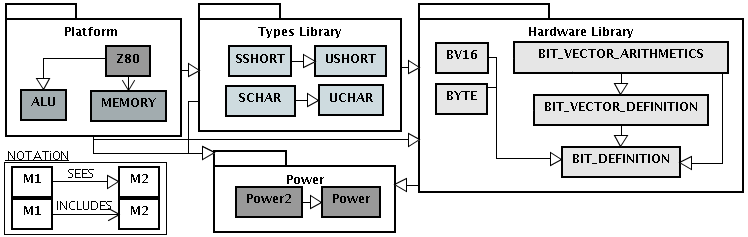
\includegraphics[width=.87\textwidth]{diagramaEstrutural_vertical_ProB2.png}
 \caption{Dependency diagram of the Z80 model.}
\label{fig:hardware-definition-graph}
\end{figure}




%[[Colocar uma breve ligação e SINTESE SOBRE A VERIFICAÇÃO DAS BIBLIOTECAS]]
The hardware library and types library have many lemmas and conversion functions with arithmetic that may be reused to model different instruction set architectures. Each finite basic data typed defined from Hardware Library has a number of proof obligation associated: 
\textsc{bit} - 118 {\small \textsc{POs}}; \textsc{byte} - 154 {\small \textsc{POs}}; \textsc{bv16} - 75 {\small \textsc{POs}}. 
The Types Library has also a number of proof obligation associated: \textsc{uchar} -  30 {POs}; \textsc{schar} - 30 {\small \textsc{POs}}; \textsc{ushort} - 62 {\small \textsc{POs}}; \textsc{sshort}  - 62 {\small \textsc{POs}}.

Nearly 50\% of all these proof obligations are verified automatically or with few user pass\footnote{The user passes allows to filter proof tactics that aid the prover to find the proof, this is a feature provided by Atelier B.}. A large part of the proof obligations require long sessions with the interactive provers, mostly because they contain complex arithmetic expressions that the automatic provers in AtelierB have difficulty handling. 
All these 531 proof obligations were eventually verified. 

 The data types quoted are used by Z80 model and this is presented in the next section.


\section{A B model of the Z80 instruction set}
\label{sec:z80}

The Z80 is a CISC microcontroller developed by \textit{Zilog}~\cite{Z80_manual}. 
The Z80 is composed by different elements: ALU, data bus, registers of 8 and 16
bits, input/output ports and interruptions. Z80 has 158 different instructions, 
including all the 78 from the Intel 8080 microprocessor, and all of them were
formally specified in B. These instructions are classified into these categories: load and
exchange; block transfer and search; arithmetic and logical; rotate
and shift; bit manipulation; jump, call and return; input/output; and
basic cpu control. Each category of instruction has different elements
of specification.

The main elements are specified in the microcontroller module Z80 and parts of it are presented here.  Basically, the
microcontroller state is formed by the program counter, ports,
registers and memory. The state transition occurs either as an instruction
execution or an external action. Groups of registers ($rgs8$, $pc$, $r\_$) are represented
by the variables of the specification states that appear in clause
\textit{VARIABLES}. The declaration of valid states of variables is in
the \textit{INVARIANT} clause and the initial state is defined in the
\textit{INITIALISATION} clause. The assembly instructions and external actions are defined
by the clause \textit{OPERATIONS} and, in general, each instruction
has three actions: update the program counter ($pc$), update the flag
register and its main effect.
% Several functions were created to Z80.
The functions specific to the microcontroller are defined in the ALU
(arithmetic logic unit) module. The main module Z80 includes an instance of
the memory module and accesses the definitions from basic data types
modules and the \textit{ALU} module.


\subsection{Modeling the actions and instructions}
%TODO: Fiz uma breve alteração
Each instruction and external action are represented by a B operation in Z80 module. 
The instruction $\textit{LD\_nn\_A}$ uses the $\textit{updateAddressMem}$
operation from \textit{Memory} module, it receives an address memory
and its new memory value. $\textit{LD\_nn\_A}$ also increments the
program counter ($\textit{pc}$) and updates the refresh register ($\textit{r\_}$). \\


\bf LD\_\(nn\)\_A  \rm =

\hspace*{0.20in}\bf PRE \it nn $\in$ \it USHORT\hspace*{0.15in} %$\land$ \hspace*{0.10in}\it nn\hspace*{0.10in} $\in$  \it DATA\_R\_ADR \hspace*{0.10in}
\bf THEN

\hspace*{0.20in}\bf updateAddressMem \rm ( \it ushort\_bv16 \rm ( \it nn \rm ) \rm , \it rgs8 \rm ( \it a0 \rm )
\rm )  $\para$

\hspace*{0.20in}\it pc \rm := \it instruction\_next \rm ( \it pc \rm )  $\para$  \it r\_ \rm := \it update\_refresh\_reg\rm (\it r\_\rm )

\hspace*{0.00in}\bf END\rm 
\\

The external actions change the state of the microcontroller, for
example, refreshing the I/O ports and requesting interruptions. The
external actions are named with the prefix ``$ext\_$'' and followed by
the name of action. There are four external actions: $ext\_update\_io\_ports$, $ext\_NMI$ and
$ext\_INT$, $ext\_Reset$. The action $ext\_update\_io\_ports$
just changes the state of I/O port,  see. \\


\hspace*{0.00in}\bf ext\_update\_io\_ports\rm (\it address\rm ,\it value\rm )\rm =

\hspace*{0.20in}\bf PRE \it address  $\in$  \it UCHAR  $\land$ \hspace*{0.10in}\it value  $\in$  \it SCHAR \bf THEN

\hspace*{0.20in}\it io\_ports \rm ( \it uchar\_byte \rm ( \it address \rm ) \rm ) \rm := \it schar\_byte \rm ( \it
value \rm )

\hspace*{0.00in}\bf END\rm
\\

The other external actions are related to interrupts. Interrupts allow
devices to suspend a routine from CPU and start a service routine.
These actions allow to exchange data or signals between CPU and external
devices. When it finishes, then the CPU comes back to the interrupted
routine. 

The interruptions  $ext\_NMI$, $ext\_INT$ and $ext\_Reset$
were specified in Z80 model, see a short description.  $ext\_NMI$ - Non-maskable interrupts cannot be disabled
by the programmer. Then, when a device makes a request, the stack pointer is pushed,
the program counter receives $66H$ (102 in decimal), the register $\textit{iff2}$ stores
$\textit{iff1}$, the register $\textit{iff1}$ resets and the refresh register is updated.
$ext\_INT$ - Maskable Interrupt is usually reserved for important functions
that can be enabled and disabled by the programmer. When a maskable interrupt
action happens, both register $\textit{iff1}$ and $\textit{iff2}$ are cleared,
disabling the interrupts, the stack pointer is pushed, the refresh register is updated and
the other effects depend on the interrupt mode register (\it im\rm).
$ext\_Reset$  - This just resets the registers related to the interruptions. Modeling details can be consulted in public project's repository.


\subsection{Verification and validation}
% OK -> como as regras foram utilizadas ? 

The model presented in this paper is suitable both for validation
through animation with ProB, and for verification through the standard
proof obligations generated by the application of the B method.

The animation in ProB is not as fast and practical as a simulation
with a dedicated tool (e.g. \cite{Simulator_z80}). ProB is a
general-purpose animator of formal specification, and addresses
computationally more difficult problems than a simulator. It is anyway
capable of animating, and also possibly model checking, a formal model
of the instruction set of the Z80, which was our initial motivation in
constructing that model. One may simulate step-by-step sequences of
Z80 instructions and visualize the visited states of ports, memory and
registers. It is a useful tool to debug by creating a trace of the
visited states, offering to analyse constants, functions and
expressions, and search possible violations. Furthermore, the expression
evaluator of ProB is very useful to analyse quickly properties related to binary arithmetic.

We had a previous experience verification in \cite{Valerio_SBMF09} with
a similar effort, where we were able to discharge all the proof obligations: 
that of the model of the Z80 instruction set designed without restricting
ourselves to constructs that may be animated with ProB, and without
modeling external actions. In that first experience, the verification took us about two
months. In the actual project, we have been able to verify 3062
(e.g. roughly 80 \%) of 3631 proof obligations in one week.



\section{Related work}
\label{sec:relatedworks}

There exists several approaches to model hardware and instruction sets
using B, not to mention other formal modelling approaches.  The paper
\cite{springerlink:Yuan2011} reports a method to specify, design and
construct sound and complete instruction set models by stepwise
refinement and formal proof using Event-B. It also discusses desirable
properties of an instruction set model. However, our work
\cite{Valerio_SBMF09} and \cite{Subotic2010} use the B method, that
seems more appropriated to software development, because it has an
implementable language defined, called B0, a model-driven approach
\cite{Dantas_SBMF08} to develop software from the functional
specification level down to assembly, and tools to convert the models
to a programming language.

A related experience on using B in the design of secure
micro-controllers is present in \cite{Marc20113}. It tries to show the
feasibility of such a technique for high confidence trustful
devices. The work \cite{Subotic2010} describes a similar approach with
MIPS CPU architecture and it shows how the CPU is formally specified
and implemented using the B method.




 
\section{Conclusions}
\label{sec:conclusions} 

% Um pequeno resumo do trabalho
This work has shown an approach to the formal modeling of the
instruction set of microcontroller using the B method.  During the
construction of this model, some problems were found in the official
reference for Z80 microcontroller~\cite{Z80_manual}. We have consulted
different sources \cite{Simulator_z80,Z80_manual} to
avoid such problems in modeling and have developed a case study: a
verified embedded software.  This case study was interesting too as a
feasibility analysis of the approach to derive formally assembly code
from a specification of functional requirements in the B method.

%TODO: COLOCAR AQUI OS PRINCIPAIS BENEFÍCIOS PROPORCIONADOS PELO TRABALHO

% fundamenta melhor o trabalho já desenvolvido. Citar o artigo SBMF e a dissertação. 
% Os meus trabalhos j√° desenvolvidos/ resultados atuais.
The following works are directly related to the objective this paper.
A first case study for this approach was reported in~\cite{Dantas_SBMF08}, presenting
more details as well as a small software that developed up to assembly
level in three different platforms. A short general view of a previous work
were presented in~\cite{Valerio_SBMF09}. The model presented in the 
current paper added support for animation in ProB and the representation
of external actions.
%Link com o par√°grafo anterior 
This set of papers presents an alternative step to software verification
up to assembly language, showing the current difficulties and
suggesting improvements in tools supporting the B method.

In the future, we plan to improve the support for the development of
software with the B method from functional specification to assembly
level, using the Z80 model presented in this work. For instance, the
mechanic compilation from B algorithmic constructs to assembly
platform is also envisioned. Finally, another important activity is to
develop a formal model of the internal representation used in LLVM
Compiler~\cite{DBLP:conf/cgo/LattnerA04}, which would enable us to
integrate different compilation techniques into our B-based framework.


\textbf{Acknowledgements:} The animation of the model would not
have been possible without the help of Michael Leuschel who kindly
provided feedback.% and developed improvements to ProB to meet our
%needs.

\bibliographystyle{plain}
\bibliography{paper}


\end{document}

